\begin{figure*}[ht]
    \vspace{-10pt}
    \begin{minipage}[b]{\textwidth}
        % \begin{center}

        \subfigure[aligned MHC pangenome]{
            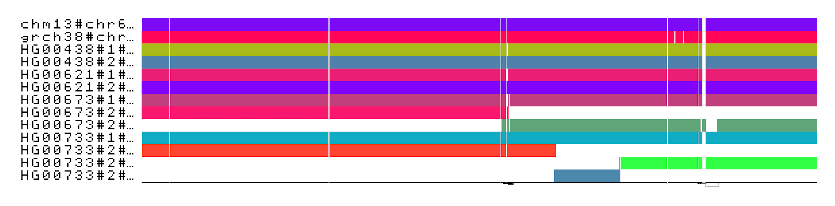
\includegraphics[width=.48\textwidth]{fig/mhc-align.eps}
            \label{fig:1a}
        }
        \vspace{-11pt}
        % \newline
        \subfigure[consensus MHC pangenome]{
            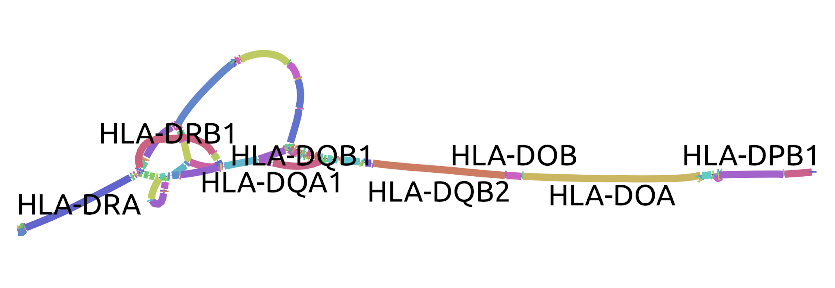
\includegraphics[width=.48\textwidth]{fig/mhc-pangenome.eps}
            \label{fig:1b}
        }
        \caption{Visualizing the Major Histocompatibility Complex (MHC) \textit{locus}.
            (a) projection of full MHC \textit{locus} of eight haploid phased human genome
            assemblies, plus the chm13 cell line and GRCh38 reference genomes, as supplied by the
            Human Reference Pangenome Consortium\citep{HRPC}, created by \cmd{odgi build+sort+viz}. The coloured
            bars represent the linearized paths, representing contigs, as a zoomed out multi-sequence
            alignment. The black lines at the bottom represent the graph topology.
            (b) consensus graph representation of the same assemblies showing variations larger than $100$ base pairs.
            The gene label coordinates were super imposed by using \cmd{odgi position} from GRCh38.
            Figure generated by the Bandage tool\citep{26099265}.
        }
        \label{fig:1}
        % \end{center}
    \end{minipage}
\end{figure*}
